\documentclass[class=scrbook, crop=false]{standalone}
\usepackage[subpreambles=true]{standalone}
\ifstandalone
    % ---------------------------------------------------------------------
% File Import Support
% ---------------------------------------------------------------------
\usepackage{import} % Enables relative path imports for modular document structure.

% ---------------------------------------------------------------------
% Language and Character Encoding
% ---------------------------------------------------------------------
\usepackage[ngerman, english]{babel} % Set document languages: German + English.

% ---------------------------------------------------------------------
% Font Configuration — LuaLaTeX Only
% ---------------------------------------------------------------------
% LuaLaTeX handles UTF-8 input natively — inputenc and fontenc are obsolete here.

\usepackage{lmodern}   % Default serif/monospace fallback fonts.
\usepackage{fontspec}  % Primary font package for LuaLaTeX.
\setsansfont{Liberation Serif}    % Set sans-serif font to Arial (main font for this document).

% Notes:
% - lmodern fills in main and monospace fonts if not explicitly set with fontspec.
% - Comment lmodern if full fontspec control is preferred.

% ---------------------------------------------------------------------
% Page Layout and Formatting
% ---------------------------------------------------------------------
\usepackage[automark,headsepline]{scrlayer-scrpage} % Header/footer management.

\newcommand{\theBCOR}{15mm} % Binding correction for double-sided print layouts.

\usepackage[
    bindingoffset=\theBCOR,
    % showframe, % Show boxes which indicate margins and paddings
    bottom = 3.5cm,
    left = 2.5cm,
    right = 2.5cm
]{geometry} % Custom page dimensions.

\usepackage{float}          % Prevent page breaks inside figures/tables.
\usepackage{pdflscape}      % Landscape page support.
\usepackage{threeparttable} % Table notes support.
\usepackage{booktabs}       % Improved table rules and spacing.

% ---------------------------------------------------------------------
% Content Presentation
% ---------------------------------------------------------------------
\usepackage{tikz}          % Graphics and diagrams.
\usepackage{graphicx}      % Image inclusion.

\addtokomafont{disposition}{\rmfamily} % Roman font for all section headings.

\usepackage[onehalfspacing]{setspace}  % Line spacing: 1.5x for readability.

\usepackage[stretch=10]{microtype}     % Typographic optimizations.
% Disable expansion if font glitches occur:
% \usepackage[stretch=10, expansion=false]{microtype}

\usepackage{textcomp}      % Access to symbols like \textmu (µ).

\usepackage[
    range-units=single,
    range-phrase=-,
    separate-uncertainty=true,
    multi-part-units=repeat
]{siunitx} % Scientific units, uncertainty handling.
% https://tex.stackexchange.com/questions/124488/multi-part-numbers-and-units-in-siunitx

\usepackage{listings}      % Source code formatting.
\usepackage{enumitem}      % Fine-tune list spacing and indentation.
\setlist{nosep}

\usepackage{todonotes}     % Inline ToDo notes.
\setuptodonotes{inline, inlinepar}
\reversemarginpar          % Place ToDo notes in the left margin.
% Adjust margin width if notes overflow:
% \setlength{\marginparwidth}{2cm}

\usepackage{xcolor}        % Color customization support.
\usepackage{amsmath}       % Math typesetting.

% ---------------------------------------------------------------------
% Utility Packages
% ---------------------------------------------------------------------
\usepackage{blindtext}     % Filler text for layout development.
\usepackage[hidelinks]{hyperref} % Hide link borders in PDF output.

% ---------------------------------------------------------------------
% Glossary and Index
% ---------------------------------------------------------------------
% IMPORTANT: Version pin required for compatibility.
\usepackage[acronym, nogroupskip]{glossaries}[=v4.49]
\usepackage{xltabular}     % Required table layout extension for glossaries.

% ---------------------------------------------------------------------
% Bibliography Configuration
% ---------------------------------------------------------------------
\usepackage{csquotes}      % Quotation style integration.
\usepackage[
    style=ieee,
    citestyle=numeric-comp,
    backend=biber
]{biblatex}

% ---------------------------------------------------------------------
% Chair specific Packages — Automatically enabled via \selectchair
% ---------------------------------------------------------------------
\ifchair{SYSCOP}
    \usepackage{optidef} % Package to write optimization problems
    \usepackage{amsfonts} % extended set of fonts for use in mathematics
\fi

% ---------------------------------------------------------------------
% Paths and Included Files
% ---------------------------------------------------------------------
% Fix paths for standalone compiling
\ifstandalone
    \def \home {..}
\else
    \def \home {.}
\fi

\input{\home/settings+/style/page}     % Page style configuration.
\graphicspath{{\home/images/}}         % Default image path.

\input{\home/settings+/style/code.tex} % Code listings style.
\lstset{inputpath={\home/code/}}       % Default path for listings files.

\input{\home/settings+/style/symbols}       % Set path to symbols list style file
\input{\home/settings+/style/acronyms}      % Set path to acronym list style file
\input{\home/references/glossary_acronyms}  % Load glossary, symbol and acronyms list

\addbibresource{\home/references/references.bib}
\input{\home/settings+/variables}

\usepackage[listings=false]{scrhack} % Compatibility fix for older packages.

% ---------------------------------------------------------------------
% Optional Packages — Comment/Uncomment As Needed
% ---------------------------------------------------------------------
% \usepackage{amsfonts}      % Additional mathematical fonts
% \usepackage{caption}       % Customize caption appearance for figures and tables
% \usepackage{subcaption}    % Create subfigures/subtables with individual subcaptions
% \usepackage{calc}          % Arithmetic with LaTeX lengths.
% \usepackage{imakeidx}      % Index creation.
% \usepackage{paralist}      % Compact lists.
% \usepackage{epigraph}      % Quotation formatting.
\usepackage{algorithm}     % Algorithms (floating).
\usepackage{algpseudocode} % Pseudocode formatting.
% \usepackage{algorithmic}   % Legacy pseudocode.
% \usepackage{xspace}        % Smart space insertion.
% \usepackage{tabularx}      % Flexible table widths.
% \usepackage{longtable}     % Multipage tables.
% \usepackage{verbatim}      % Multiline comments.
% \usepackage{datapie}       % Pie charts.
% \usepackage{afterpage}     % Command placement after page breaks.
% \usepackage{wrapfig}       % Text wrapping around figures.
\usepackage{amsthm}
\usepackage{graphicx}
\usepackage{subcaption}
\usepackage{nicematrix}

\theoremstyle{plain}
\newtheorem{remark}{Remark}
\newtheorem{assumption}{Assumption}
\newtheorem{theorem}{Theorem}
\newtheorem{lemma}[theorem]{Lemma}
\newtheorem{proposition}[theorem]{Proposition}
\fi

% ----------------------------------------------------------------------------
%                               Implementation
% ----------------------------------------------------------------------------
\begin{document}

\chapter{A benchmark for indefinite OCP QPs} % Outline text
\label{Chapter::Benchmark}
In order to evaluate the performance of the proposed Riccati-based primal regularization, 
especially in the context of the subproblems of \gls{SQP},
in this chapter, we aim at constructing a benchmark of indefinite \gls{OCP} \glspl{QP} that arise in the \gls{SQP} iterations of \gls{NMPC} problems.
We will first introduce the construction of the \gls{QP} benchmark, 
including the formulation of \gls{QP} subproblems in the benchmark, an overview of \gls{OCP} test problems 
and the pipeline for collecting indefinite \glspl{QP} in Section \ref{sec:benchmark_construction}.
Then we will analyze the collected problem instances to gain a better understanding of characteristics
regarding definiteness in the indefinite \gls{OCP} \gls{QP} benchmark in Section \ref{sec:benchmark_analysis}.

\section{Benchmark construction}
\label{sec:benchmark_construction}
This section describes the construction of the indefinite \gls{QP} benchmark.
We first formulate the \gls{QP} subproblems arising in the \gls{SQP} iterations of the \glspl{OCP},
then introduce the eight \gls{OCP} test problems,
formulated as fixed-time regulator problems with quadratic stage costs and box constraints on the controls,
and finally the collection pipeline.

\subsection{Formulation of QP subproblems from OCPs}
\label{subsec:formulation}
We will start from the formulation of the nonlinear \glspl{OCP} to obtain the resulting \gls{QP} subproblems that arise in the \gls{SQP} iterations.
In the benchmark, all \glspl{OCP} share the same structure: 
a fixed-horizon, direct multiple-shooting \gls{OCP} 
with a quadratic stage cost that penalizes deviations from given state and control references.
The mathematical formulation of the \glspl{OCP} is given as follows:
\begin{mini}[2]
    {x, u}
    {\sum_{k=0}^{N-1} \frac{1}{2}
        \begin{bmatrix} x_k-x_k^{\mathrm{ref}} \\ u_k-u_k^{\mathrm{ref}} \end{bmatrix}^{\!\top}
        \begin{bmatrix} \mathcal{Q}_k & \mathcal{S}_k^{\top} \\ \mathcal{S}_k & \mathcal{R}_k \end{bmatrix}
        \begin{bmatrix} x_k-x_k^{\mathrm{ref}} \\ u_k-u_k^{\mathrm{ref}} \end{bmatrix}}
    {\label{eq:ocp}}
    {}
    \breakObjective{+ \tfrac12\|x_N-x_N^{\mathrm{ref}}\|_{\mathcal{Q}_N}^2}
    \addConstraint{x_0}{= \bar{x}_0}
    \addConstraint{x_{k+1}}{= f_k(x_k,u_k),\quad}{k = 0, \ldots, N-1}
    \addConstraint{\underline{g}}{\le \mathcal{C}_k x_k + \mathcal{D}_k u_k \le \bar{g},}{k = 0, \ldots, N-1}
    \addConstraint{\underline{h}}{\le h_k(x_k,u_k) \le \bar{h},}{k = 0, \ldots, N-1}
    \addConstraint{\underline{g}_N}{\le \mathcal{C}_N x_N \le \bar{g}_N,}
\end{mini}

where $x_{k+1}=f_k(x_k,u_k)$ is one integration step of the continuous dynamics over $[t_k,t_{k+1}]$.
$\bar{x}_0$ is the given initial state,
$\mathcal{Q}_k,\mathcal{R}_k,\mathcal{Q}_N\succeq 0$ are weighting matrices, 
$\mathcal{S}_k$ is the coupling cost matrix,
and $x_k^{\mathrm{ref}},u_k^{\mathrm{ref}}$ are the reference points. 
$\mathcal{C}_k x_k + \mathcal{D}_k u_k$ includes the affine and box path constraints,
$h_k(\cdot, \cdot)$ collects the nonlinear path constraints,
and $\underline{g}_N \le \mathcal{C}_N x_N \le \bar{g}_N$ are the terminal inequality constraints.

When using the exact Hessian of the Lagrangian in the \gls{SQP} iterations, the resulting Hessian of the \gls{QP} subproblem at stage $k = 0, \dots, N-1$ reads:
\begin{align}
    H_k &= \nabla^2 \mathcal{L}(x, u, \pi, \lambda)  \notag \\
        &= \begin{bmatrix} \mathcal{Q}_k & \mathcal{S}_k^{\top} \\ \mathcal{S}_k & \mathcal{R}_k \end{bmatrix} + \sum_{j=1}^{n_x} (\pi_k)_j \nabla^2 [f_k]_j(x_k,u_k) + \sum_{j=1}^{n_c} (\lambda_k)_j \nabla^2 [h_k]_j(x_k,u_k),
\end{align}
where $n_x$ is the dimension of states and $n_c$ is the number of nonlinear constraints, 
$\pi_k$ and $\lambda_k$ are the Lagrange multipliers associated with the dynamics and nonlinear constraints, respectively.

The definiteness of $H_k$ is thus determined by two parts,
a constant cost block  $\left[\begin{smallmatrix}\mathcal{Q}_k & \mathcal{S}_k^{\top}\\ \mathcal{S}_k & \mathcal{R}_k\end{smallmatrix}\right]$
and an iterate-dependent cost from the two curvature terms.
In the latter, each component Hessian $\nabla^2[f_k]_j$ and $\nabla^2[h_k]_j$ is symmetric but carries no definiteness guarantee, 
and the associated multipliers $(\pi_k)_j$ and $(\lambda_k)_j$ may take arbitrary sign and magnitude during the \gls{SQP} iterations.

The weighted sum $H_k$ is thus a general symmetric and typically indefinite matrix, in particular when the multipliers are large.
Consequently, the exact-Hessian \gls{QP} subproblem is in general nonconvex.

As for $H_N$, neither the dynamics nor the affine terminal constraints add curvature in $x_N$,
so $H_N = \mathcal{Q}_N \succeq 0$ is constant.

Collecting the stage Hessians $H_k$ and Jacobians and linearizing the constraints of~\eqref{eq:ocp} at the current \gls{SQP} iterate yields a
structured \gls{QP}. The subproblem takes the form:
\begin{mini}[2]
    {\Delta x, \Delta u}
    {\sum_{k=0}^{N-1} \left( \frac{1}{2}
        \begin{bmatrix} \Delta x_k \\ \Delta u_k \end{bmatrix}^{\!\top}
        \begin{bmatrix} Q_k & S_k^\top \\ S_k & R_k \end{bmatrix}
        \begin{bmatrix} \Delta x_k \\ \Delta u_k \end{bmatrix}
        + \begin{bmatrix} q_k \\ r_k \end{bmatrix}^{\!\top}
        \begin{bmatrix} \Delta x_k \\ \Delta u_k \end{bmatrix} \right)}
    {}
    {}
    \breakObjective{+ \tfrac{1}{2}\, \Delta x_N^\top Q_N\, \Delta x_N + q_N^\top \Delta x_N}
    \addConstraint{\Delta x_0}{= \Delta \bar{x}_0}
    \addConstraint{\Delta x_{k+1}}{= A_k \Delta x_k + B_k \Delta u_k + c_k,\quad}{k = 0, \ldots, N-1}
    \addConstraint{\begin{bmatrix} \underline{u}_k \\ \underline{x}_k \\ \underline{d}_k \end{bmatrix}}
        {\le \begin{bmatrix} J_k^{b,u} & 0 \\ 0 & J_k^{b,x} \\ D_k & C_k \end{bmatrix}
        \begin{bmatrix} \Delta u_k \\ \Delta x_k \end{bmatrix}
        \le \begin{bmatrix} \overline{u}_k \\ \overline{x}_k \\ \overline{d}_k \end{bmatrix},}
        {k = 0, \ldots, N-1}
    \addConstraint{\underline{\Delta x}_N}{\le J_N^{b,x} \Delta x_N \le \overline{\Delta x}_N,}
\end{mini}
where, at each stage $k$, $\Delta x_k \in \mathbb{R}^{n_x}$ and $\Delta u_k \in \mathbb{R}^{n_u}$
denote the state and control deviation variables, and $N$ is the horizon length.

All remaining quantities are obtained by linearizing the \gls{OCP} at the
current \gls{SQP} iterate $(x_k,u_k)$ with multipliers $(\pi_k,\lambda_k)$:
\begin{itemize}
    \item $Q_k$, $R_k$, and $S_k$ are the state, control, and coupling blocks of the exact Lagrangian Hessian $H_k$.
    $q_k=\mathcal{Q}_k(x_k-x_k^{\mathrm{ref}})+\mathcal{S}_k^{\top}(u_k-u_k^{\mathrm{ref}})$ and 
    $r_k=\mathcal{R}_k(u_k-u_k^{\mathrm{ref}})+\mathcal{S}_k(x_k-x_k^{\mathrm{ref}})$ are the corresponding stage-cost gradients, 
    and $Q_N$, $q_N$ are the terminal Hessian and gradient.

    \item $A_k=\nabla_{x_k} f_k$ and $B_k=\nabla_{u_k} f_k$ are the Jacobians of the discretized dynamics,
    and $c_k=f_k(x_k,u_k)-x_{k+1}$ is the dynamics residual at the current iterate. 
    At a dynamically feasible iterate $c_k=0$.

    \item $\Delta\bar{x}_0=\bar{x}_0-x_0$ is the residual of the initial equality constraint,
    i.e.\ the solution needed to satisfy $x_0=\bar{x}_0$ after the step.

    \item $J_k^{b,u}$ and $J_k^{b,x}$ are selection matrices picking out the bounded control and state components for box constraints,
    with bounds $\underline{u}_k,\overline{u}_k$ and $\underline{x}_k,\overline{x}_k$.

    \item $C_k=\left[\begin{smallmatrix}\mathcal{C}_k\\ \nabla_{x_k} h_k\end{smallmatrix}\right]$ and
    $D_k=\left[\begin{smallmatrix}\mathcal{D}_k\\ \nabla_{u_k} h_k\end{smallmatrix}\right]$ stack the Jacobians of the affine and nonlinear path constraints,
    with $\underline{d}_k=\left[\begin{smallmatrix}\underline{g}-\mathcal{C}_k x_k-\mathcal{D}_k u_k\\ \underline{h}-h_k(x_k,u_k)\end{smallmatrix}\right]$ and
    $\overline{d}_k=\left[\begin{smallmatrix}\bar{g}-\mathcal{C}_k x_k-\mathcal{D}_k u_k\\ \bar{h}-h_k(x_k,u_k)\end{smallmatrix}\right]$;
    these constraints couple states and controls.
\end{itemize}

\subsection{Benchmark OCPs}
In this subsection, we introduce the eight \glspl{OCP} used to construct the benchmark. 
Each \gls{OCP} is based on a dynamic system provided in~\cite{Kiessling2026} 
and formulated as a regulation or point-to-point transfer problem with problem-specific modifications, 
which can be uniformly described with \eqref{eq:ocp}.
The eight \glspl{OCP} are named and characterized as follows:
\begin{itemize}
    \item \textbf{Pendulum:} An inverted pendulum on a cart, actuated by a horizontal force.
    It is steered from the downward to the upright equilibrium under an input bound and a mixed state--input constraint.
    The stage cost contains a bilinear state--input term, which makes indefinite Hessians more likely.
    \item \textbf{Acrobot:} Adapted from \cite{spong1995swing}.
    A two-link pendulum with joint friction, actuated only at the elbow.
    Terminal equality constraints drive it between two prescribed configurations, an underactuated and strongly nonlinear maneuver.
    \item \textbf{Dubins car:} Adapted from \cite{dubins1957curves}.
    A kinematic unicycle with position and heading as states and forward velocity and turn rate as inputs.
    It performs a parallel-parking maneuver in a narrow corridor given by state bounds, with a terminal equality constraint on the full pose.
    \item \textbf{Furuta:} Adapted from \cite{furuta1992swing}.
    A rotary inverted pendulum with identified parameters and joint damping, actuated by a single torque on the base arm.
    The pendulum is swung up and stabilized upright under tight torque limits on a non-uniform time grid.
    \item \textbf{Flying robot:} Adapted from \cite{betts2010practical}.
    A planar free-flying robot driven by four nonnegative thrusters, which produce a net force along the body axis and a turning moment.
    It is steered to zero position and orientation with a prescribed translational velocity, under linear constraints on the summed thrust.
    \item \textbf{Robot arm:} Adapted from \cite{betts2010practical}.
    A three-degree-of-freedom arm (radial extension, rotation, elevation) with configuration-dependent inertia
    and a cross-axis actuator coupling that is nonlinear in the inputs.
    One joint angle is moved to a new set-point under state and input bounds; the input coupling makes the exact Hessian indefinite.
    \item \textbf{Crane:} Adapted from \cite{betts2010practical}.
    An overhead crane with hoisting length, trolley position and swing angle as states, actuated by trolley and hoisting accelerations.
    The load is moved between two rest positions under a swing-rate bound and a nonlinear constraint on the payload region.
    \item \textbf{Moonlander:} Adapted from \cite{meditch1964optimal}.
    A planar lunar lander with translational and rotational motion under reduced gravity, actuated by two laterally offset thrusters.
    It lands softly on a ground target with zero terminal velocity under nonnegative, bounded thrust.
\end{itemize}

\begin{table}[htbp]
    \centering
    \caption{Summary of the evaluated \glspl{OCP}. The state dimension
    $n_x$, control dimension $n_u$, and horizon length $N$ span a range
    of common control problem scales.}
    \label{tab:ocp_problems}
    \begin{tabular}{l ccc}
        \toprule
        \textbf{Problem} & $n_x$ & $n_u$ & $N$ \\
        \midrule
        Pendulum     & 4 & 1 & 25 \\
        Acrobot      & 4 & 1 & 15 \\
        Dubins car   & 3 & 2 & 25 \\
        Furuta       & 4 & 1 & 20 \\
        Flying robot & 6 & 4 & 50 \\
        Robot arm    & 6 & 3 & 30 \\
        Crane        & 6 & 2 & 40 \\
        Moonlander   & 6 & 2 & 30 \\
        \bottomrule
    \end{tabular}
\end{table}

Besides the different physical systems,
these \glspl{OCP} also cover different state and control dimensions, as shown in Table \ref{tab:ocp_problems}. 
The state dimension $n_x$ ranges from $3$ to $6$, the control dimension $n_u$ from $1$ to $4$, and the horizon length $N$ from $15$ to $50$.
This spread is chosen so that the benchmark spans a range of common problem scales in control problems.

\subsection{Collection pipeline}
Based on the eight \glspl{OCP}, 
we can construct a benchmark of indefinite \glspl{QP} arising from \gls{SQP}-based \gls{NMPC}. 
Specifically, we establish a collection pipeline that extracts the \gls{QP} subproblems directly from intermediate \gls{SQP} iterations.
The collection pipeline consists of two steps: \emph{generate} and \emph{collect}, and can be summarized as follows:

\begin{enumerate}
    \item \textbf{Generate:} In this step, we generate iterates by solving the \gls{OCP} with \gls{SQP} 
    and obtain iterates from early to late \gls{SQP} iterations.
    To keep the \gls{SQP} iterations from failing on indefinite exact-Hessian \glspl{QP}, 
    we use \gls{SQP}-level regularization or the Gauss--Newton Hessian approximation in \texttt{acados}.

    \item \textbf{Collect:} In this step, 
    we utilize the previously generated iterates as initial guesses for linearization within the solver. 
    We can selectively collect indefinite \glspl{QP} that exhibit an indefinite reduced Hessian.
\end{enumerate}

In the collect step, all \glspl{QP} share one failing status code from \texttt{acados}, code \texttt{4} for infeasible \gls{QP},
which indicates that the indefinite reduced Hessian causes the failure of the Riccati recursion in HPIPM.
This is intentionally achieved by setting the Riccati algorithm in HPIPM as classical Riccati recursion, i.e.\ \texttt{ric\_alg = 0}, 
which requires the reduced Hessian to be \gls{PD} in order to proceed with the Riccati recursion,
instead of the square-root version \cite{frisonAlgorithmsMethodsHighPerformance}, which requires the full Hessian to be \gls{PD}.
When HPIPM fails to proceed with the Riccati recursion, it indicates that the reduced Hessian is indefinite,
and the corresponding \gls{QP} is collected.

For each problem, we limit the number of near-identical \glspl{QP},
so that the number of instances per problem stays within a comparable range and the collected instances remain meaningful.
We also use IPOPT~\cite{wachter2006implementation} as a reference solver and keep only the \glspl{QP} that it solves successfully.
After this filtering, we obtain a total of $175$ indefinite \glspl{QP} from the eight \glspl{OCP},
the per-problem counts are reported in Table~\ref{tab:collected_qps} and range from $15$ to $29$.
These \glspl{QP} are stored in JSON format and are available at \url{https://github.com/Pandatheon/Primal-dual_IPM.git}.

\begin{table}[htbp]
    \centering
    \caption{Number of indefinite QPs collected from each OCP ($175$ in total).}
    \label{tab:collected_qps}
    \begin{tabular}{l c}
        \toprule
        \textbf{Problem} & \textbf{Number} \\
        \midrule
        Pendulum     & 18 \\
        Acrobot      & 15 \\
        Dubins car   & 29 \\
        Furuta       & 19 \\
        Flying robot & 20 \\
        Robot arm    & 24 \\
        Crane        & 29 \\
        Moonlander   & 21 \\
        \bottomrule
    \end{tabular}
\end{table}

\section{Benchmark analysis}
\label{sec:benchmark_analysis}
In this section,
we will analyze the collected instances regarding the definiteness in the benchmark.
The distribution of indefiniteness is analyzed in Section \ref{subsec:distribution},
which describes the magnitude and coverage of the indefinite reduced Hessians in the collected \glspl{QP},
and the source of indefiniteness is analyzed in Section \ref{subsec:source}, 
which further illustrates the source of indefiniteness in the collected \glspl{QP} 
by analyzing the eigenvalues of the reduced Hessian blocks at each stage.

\subsection{Distribution of indefiniteness}
\label{subsec:distribution}
We first characterize the collected \glspl{QP} along two axes:
the \emph{depth} of indefiniteness, 
measured by the magnitude of the most negative eigenvalue $|\nu_{\min}|$ of the reduced Hessian,
and the \emph{width}, measured by the fraction of reduced Hessian blocks that are indefinite within a \gls{QP}.

\begin{figure}[htbp]
    \centering
    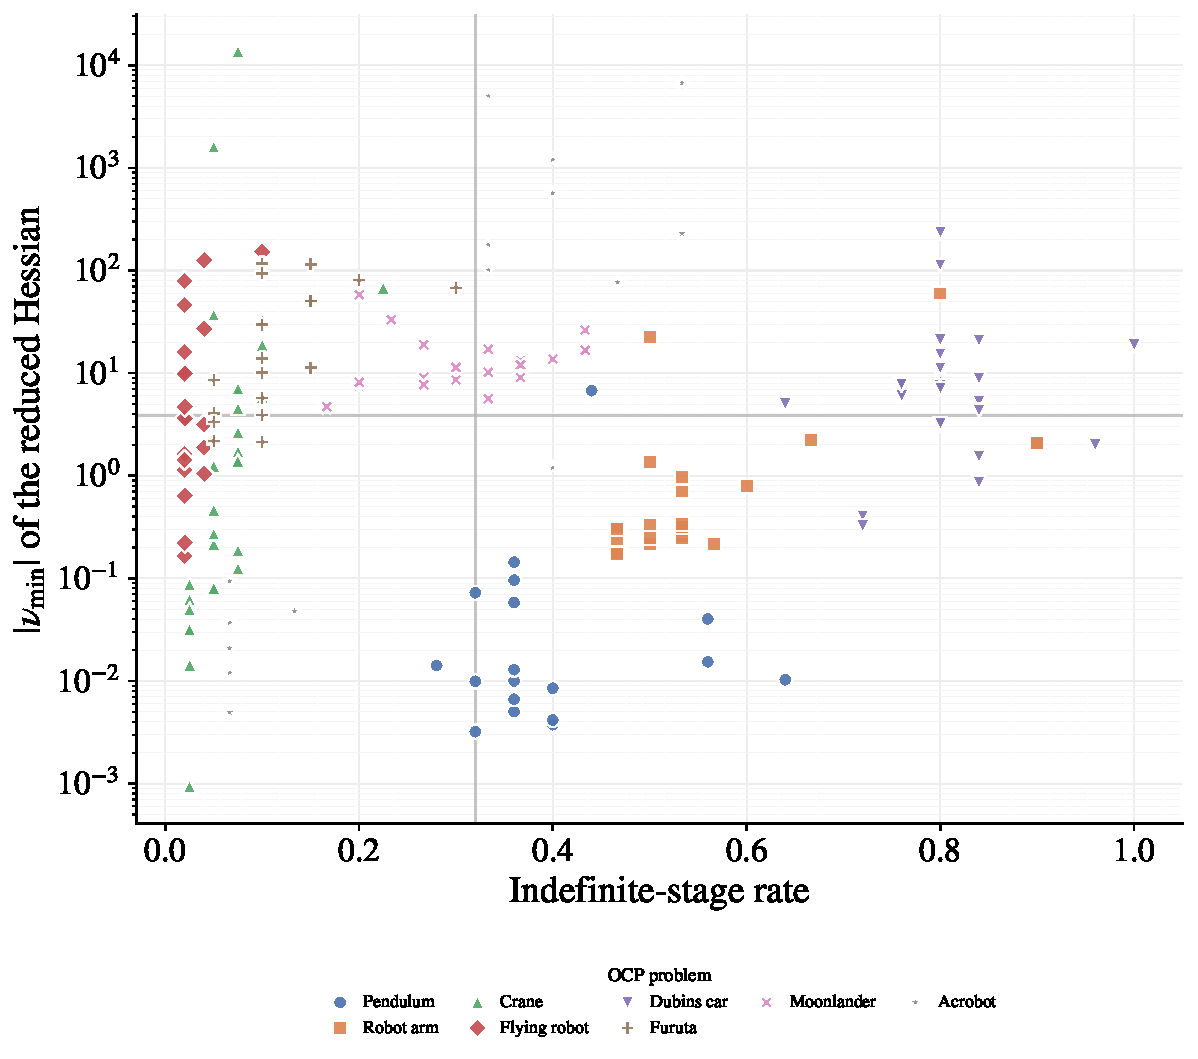
\includegraphics[width=0.95\textwidth]{images/benchmark/indefiniteness_coverage_scatter.pdf}
    \caption{Depth ($|\nu_{\min}|$ of the reduced Hessian, log scale)
    versus width (indefinite-stage rate) of the collected QPs, colored by
    OCP.}
    \label{fig:indefinite_qp_scatter}
\end{figure}

As seen from Figure~\ref{fig:indefinite_qp_scatter}, 
the depth of the collected \glspl{QP} ranges from near zero to very large values,
and each \gls{OCP} occupies its own region of the depth--width plane.
Problems that are indefinite in only a small fraction of their stages, 
such as \textsl{Crane}, \textsl{Flying robot} and \textsl{Furuta}
(indefinite-stage rates below $0.30$), can still reach deep negative curvature.
Conversely, \textsl{Dubins car} and \textsl{Robot arm}, with indefinite-stage rates from $0.47$ up to $1$, show only moderate depth.
In the collected \glspl{QP}, wide and deep indefiniteness thus seldom occur together.

\textsl{Moonlander} and \textsl{Acrobot} lie in between, with intermediate indefinite-stage rates.
\textsl{Moonlander} stays within a narrow depth band, whereas \textsl{Acrobot} spans almost the full depth range of the benchmark.
\textsl{Pendulum} contributes \glspl{QP} with very shallow negative curvature at intermediate rates.
The eight \glspl{OCP} thus cover narrow-but-deep, intermediate and wide-but-moderate indefiniteness.

\begin{figure}[htbp]
    \centering
    \begin{minipage}[t]{0.48\textwidth}
        \centering
        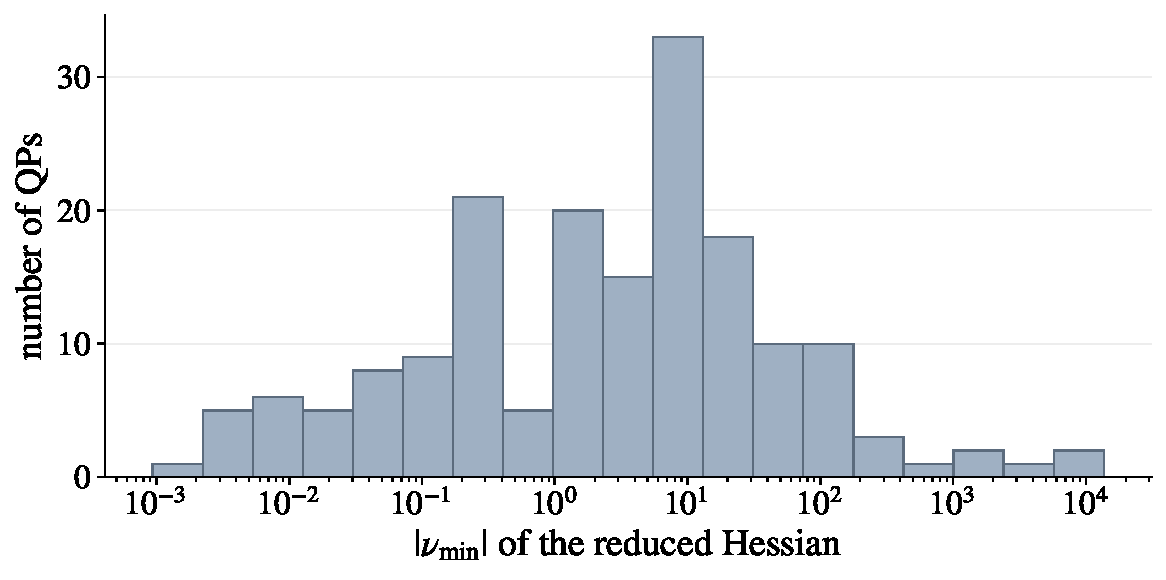
\includegraphics[width=\linewidth]{images/benchmark/indefiniteness_coverage_depth.pdf}
        \subcaption{Depth: distribution of $|\nu_{\min}|$.}
        \label{fig:indefinite_depth}
    \end{minipage}
    \hfill
    \begin{minipage}[t]{0.48\textwidth}
        \centering
        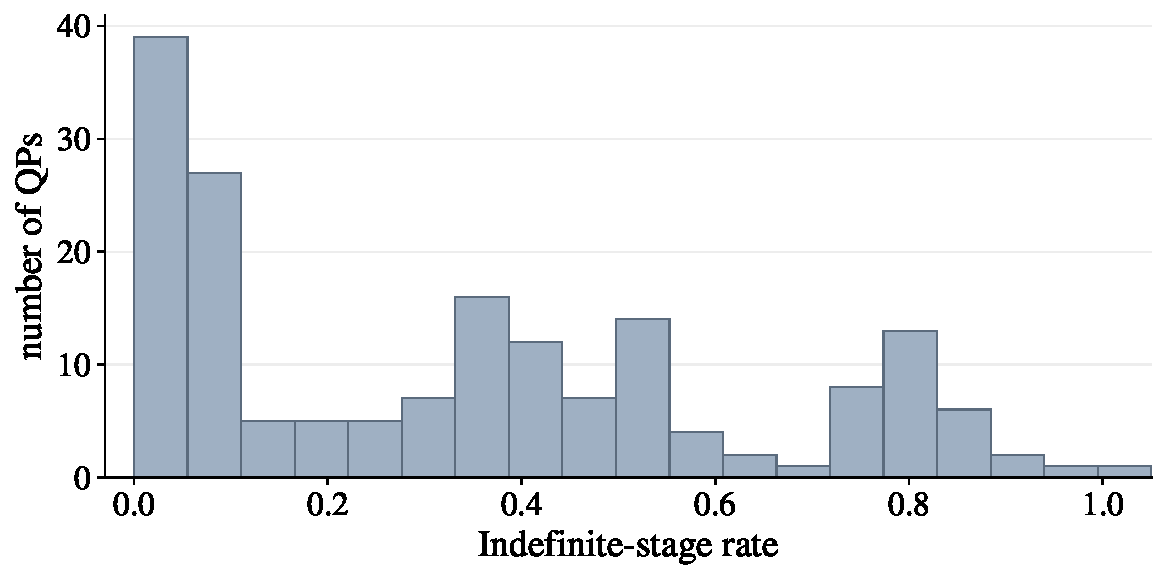
\includegraphics[width=\linewidth]{images/benchmark/indefiniteness_coverage_breadth.pdf}
        \subcaption{Width: distribution of the indefinite-stage rate.}
        \label{fig:indefinite_breadth}
    \end{minipage}
    \caption{Marginal distributions of depth and width over all collected QPs.}
    \label{fig:indefinite_marginals}
\end{figure}

Figure~\ref{fig:indefinite_marginals} shows the marginal distributions of the same data.
The depth histogram (Figure~\ref{fig:indefinite_depth}) peaks around $|\nu_{\min}| \approx 10$
and thins out towards both ends.
The negative curvature encountered during the \gls{SQP} iterations is therefore typically of moderate magnitude.
The width histogram (Figure~\ref{fig:indefinite_breadth}) covers the full range up to~$1$,
with a large share of \glspl{QP} indefinite in only a few stages, close to $40\%$.
The remaining \glspl{QP} form smaller groups at intermediate and high rates.

\subsection{Source of indefiniteness}
\label{subsec:source}
Recall that the reduced Hessian block at stage $k$, $M_k = R_k + B_k^\top P_{k+1}B_k$,
is assembled from two parts, the control cost block $R$ and the cost-to-go block $P$.

To investigate where the indefiniteness originates,
we classify every indefinite stage by which of $R_k$ and $P_{k+1}$ has a negative eigenvalue:
\emph{R only} ($R_k \not\succeq 0$, $P_{k+1} \succeq 0$),
\emph{P only} ($P_{k+1} \not\succeq 0$, $R_k \succeq 0$),
and \emph{both} ($R_k, P_{k+1} \not\succeq 0$).
Since $R_k, P_{k+1} \succeq 0$ would imply $M_k \succeq 0$, these three cases cover all indefinite stages.

Figure~\ref{fig:indefinite_source_counts} aggregates all indefinite stages across the benchmark.
In $1114$ of the $1571$ indefinite stages ($71\%$), \emph{both} $R$ and $P$ are indefinite.
Of the remaining stages, $299$ ($19\%$) are \emph{P only} and $158$ ($10\%$) are \emph{R only}.
In total, $P$ is indefinite in $1413$ stages ($90\%$) and $R$ in $1272$ ($81\%$).

\begin{figure}[htbp]
    \centering
    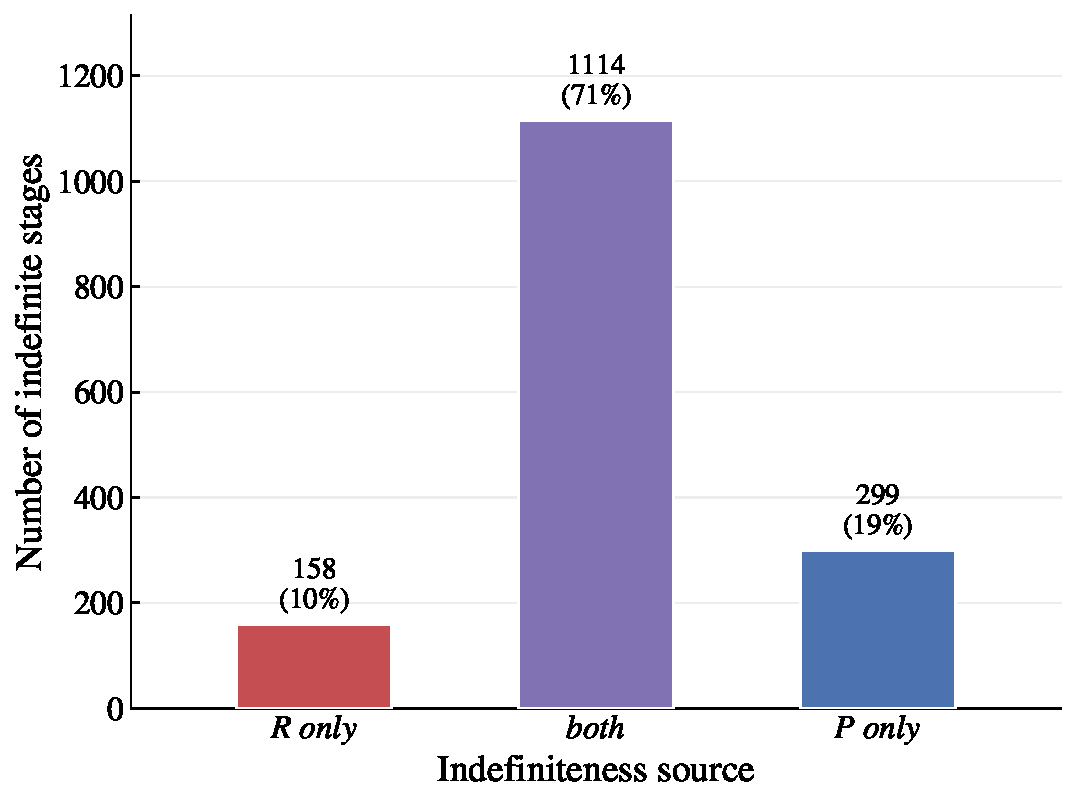
\includegraphics[width=0.7\textwidth]{images/benchmark/stage_indefiniteness_source.pdf}
    \caption{Number of indefinite stages per category, \emph{R only}, \emph{P only} or \emph{both},
    according to which of $R_k$ and $P_{k+1}$ has a negative eigenvalue.}
    \label{fig:indefinite_source_counts}
\end{figure}

\begin{figure}[htbp]
    \centering
    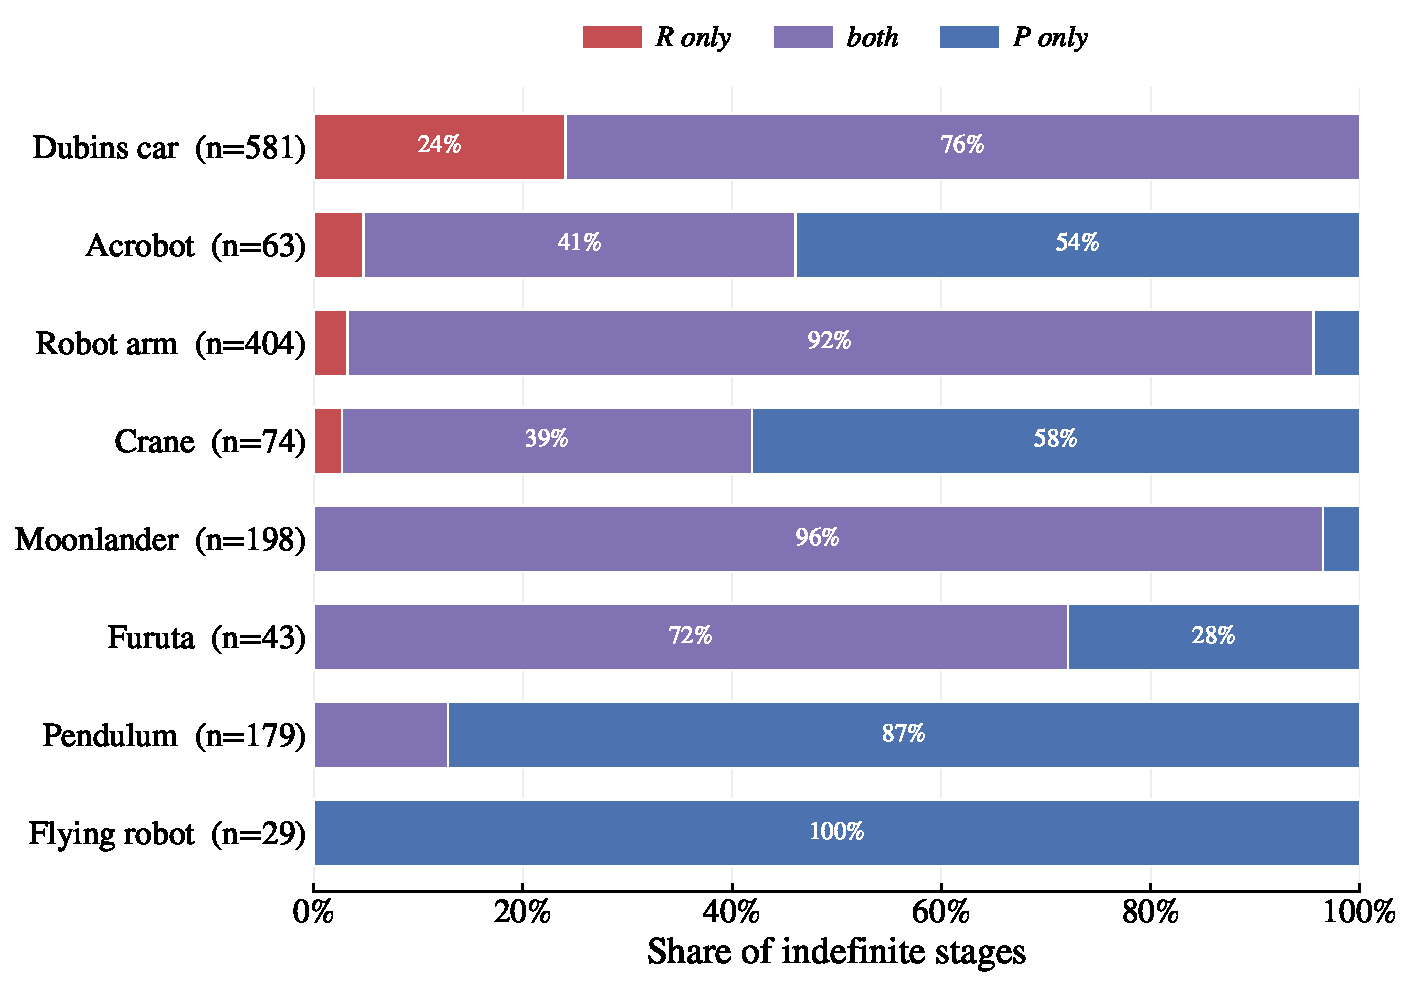
\includegraphics[width=1.0\textwidth]{images/benchmark/stage_indefiniteness_signature.pdf}
    \caption{Per-problem composition of stage indefiniteness. Each bar
    shows, for one OCP, the share of stages that are \emph{R only},
    \emph{both} and \emph{P only} ($n$ is the number of collected indefinite stages).}
    \label{fig:indefinite_source_signature}
\end{figure}

Figure~\ref{fig:indefinite_source_signature} breaks the same classification down per problem.
Six of the eight \glspl{OCP} are dominated by a single category ($\geq\!70\%$ of their stages),
and only \textsl{Acrobot} and \textsl{Crane} are mixed.

The \emph{both} case dominates \textsl{Moonlander} ($96\%$), \textsl{Robot arm} ($92\%$), \textsl{Dubins car} ($76\%$) and \textsl{Furuta} ($72\%$).
The \emph{P only} case dominates \textsl{Flying robot} ($100\%$) and \textsl{Pendulum} ($87\%$),
and is also the largest category in the two mixed problems,
\textsl{Crane} ($58\%$ against $39\%$ \emph{both}) and \textsl{Acrobot} ($54\%$ against $41\%$ \emph{both}).
The \emph{R only} case appears in four problems and is substantial only for \textsl{Dubins car} ($24\%$ of its stages),
in \textsl{Robot arm}, \textsl{Acrobot} and \textsl{Crane} it stays below $5\%$.
Among all, the \textsl{Flying robot} is the clearest case: all of its indefinite stages are \emph{P only}, 
with $R_k \succ 0$ throughout.
Its negative curvature thus enters the reduced Hessian only through the cost-to-go block, at isolated stages.

In conclusion, the cost-to-go block is involved in $90\%$ of the indefinite stages,
so a regularization strategy that merely enforces $M\succ 0$ would leave the negative curvature unaddressed in most stages.

\end{document}